% ETTCM reproduction -- module presentation (20 pages)
% Build:  cd presentation && latexmk -pdf ettcm_presentation.tex
\PassOptionsToPackage{table}{xcolor}
\documentclass[aspectratio=169,10pt]{beamer}
\usetheme[progressbar=frametitle,numbering=fraction,block=fill,sectionpage=none]{metropolis}
\usepackage[T1]{fontenc}
\usepackage{lmodern}          % Latin Modern = Computer Modern; Beamer uses its sans-serif face
\setbeamerfont{frametitle}{series=\bfseries}
\setbeamerfont{title}{series=\bfseries}
\usepackage{amsmath,amssymb,bm}
\usepackage{booktabs,multirow,array}
\usepackage{graphicx,adjustbox}
\usepackage{tikz}
\usetikzlibrary{arrows.meta,positioning,calc,shapes.geometric,decorations.pathreplacing,shadows}
\usepackage{pgfplots}
\pgfplotsset{compat=1.18}
\usepackage{fontawesome5}
\usepackage[most]{tcolorbox}
\graphicspath{{figs/}{../figures/}}

% ---------------------------------------------------------------- names
\newcommand{\presenters}{%
  \begin{tabular}{@{}ll@{}}
    \toprule
    \textbf{Name} & \textbf{Index number} \\
    \midrule
    Priyadarshana S.A.D & 230502X \\
    Perera W.A.L.S & 230487D \\
    \bottomrule
  \end{tabular}}
\newcommand{\module}{EN3160 -- Image Processing and Machine Vision}

% ---------------------------------------------------------------- colours
\definecolor{ink}{HTML}{1F2A44}
\definecolor{titlebar}{HTML}{3730AA}
\definecolor{accent}{HTML}{E00000}
\definecolor{teal}{HTML}{17A398}
\definecolor{good}{HTML}{CDEFD9}
\definecolor{mid}{HTML}{FFF0C2}
\definecolor{bad}{HTML}{F9D0C9}
\definecolor{soft}{HTML}{F3F4F7}
\setbeamercolor{frametitle}{bg=titlebar,fg=white}
\setbeamercolor{progress bar}{fg=accent,bg=titlebar!30}
\setbeamercolor{title separator}{fg=accent}
\setbeamercolor{alerted text}{fg=accent}
\setbeamercolor{block title}{bg=ink!12,fg=ink}
\setbeamercolor{block body}{bg=soft}
\setbeamercolor{normal text}{fg=ink}
\setbeamercolor{background canvas}{bg=white}

\newcommand{\G}{\cellcolor{good}}
\newcommand{\M}{\cellcolor{mid}}
\newcommand{\B}{\cellcolor{bad}}
\newcommand{\us}{\,$\mu$s}
\newcommand{\ok}{{\color{teal}\faCheck}}
\newcommand{\no}{{\color{accent}\faTimes}}
% Footnotes, research-paper style: \fnmark{*} next to the item, and one \footer{...}
% per frame (before \end{frame}) holding the notes, e.g.
%   \footer{\fnitem{*}{First note.}\quad \fnitem{\dag}{Second note.}}
\newcommand{\fnmark}[1]{\textsuperscript{#1}}
\newcommand{\fnitem}[2]{\textsuperscript{#1}\,#2}
\newcommand{\footer}[1]{%
  \begin{tikzpicture}[remember picture,overlay]
    \node[anchor=south west,inner sep=0,font=\scriptsize,text=ink,text width=0.86\paperwidth,align=left]
      (fn) at ([xshift=4mm,yshift=2.4mm]current page.south west) {#1};
    \draw[ink!45,line width=0.4pt] ([yshift=1.3mm]fn.north west) --
      ([xshift=-4mm,yshift=1.3mm]current page.south east |- fn.north);
  \end{tikzpicture}}
% Section name shown at the right of the title bar (replaces the section divider pages):
% \settag{...} before the frames of each section.
\newcommand{\sectag}{}
\newcommand{\settag}[1]{\renewcommand{\sectag}{#1}}
\addtobeamertemplate{frametitle}{}{%
  \nointerlineskip\vbox to 0pt{\hbox to 0pt{%
  \begin{tikzpicture}[remember picture,overlay]
    \node[anchor=north east,font=\scriptsize,text=white!78!titlebar,inner sep=0]
      at ([xshift=-3mm,yshift=-2.2mm]current page.north east) {\sectag};
  \end{tikzpicture}\hss}\vss}\nointerlineskip}
\renewcommand{\arraystretch}{1.12}
\newcolumntype{L}[1]{>{\raggedright\arraybackslash}p{#1}}

\newtcolorbox{card}[2][]{enhanced,colback=soft,colframe=#2,boxrule=0pt,leftrule=3pt,
  arc=2pt,left=6pt,right=6pt,top=4pt,bottom=4pt,fontupper=\small\raggedright,#1}

\title{Time-to-Contact Map from a Single Event Camera}
\subtitle{Reproducing Nunes, Perrinet \& Ieng, ICCV 2023}
\author{\texorpdfstring{\presenters}{Priyadarshana S.A.D, Perera W.A.L.S}}
\institute{\module}
\date{25 November 2026}

\begin{document}

% ================================================================= title + outline
\begin{frame}[plain,noframenumbering]
  \titlepage
  \begin{tikzpicture}[remember picture,overlay]
    \node[anchor=south east,fill=soft,rounded corners=3pt,inner sep=7pt,text width=6.4cm,
          font=\small,align=left,text=ink]
      at ([xshift=-8mm,yshift=9mm]current page.south east) {%
      {\color{titlebar}\bfseries Outline}\\[3pt]
      \begin{tabular}{@{}r@{\enspace}l@{}}
        1 & The problem \\
        2 & Why this paper is different \\
        3 & Use cases \\
        4 & Methodology \\
        5 & Experiments \\
        6 & What we did and how much we reproduced \\
      \end{tabular}};
  \end{tikzpicture}
\end{frame}

% ================================================================= 1
\section{The problem}
\settag{1\enspace The problem}

\begin{frame}{Time-to-contact: how long until we hit it?}
  \begin{columns}[T,onlytextwidth]
    \column{0.52\textwidth}
    \centering
    \begin{tikzpicture}
      \node[anchor=south west,inner sep=0] (img)
        {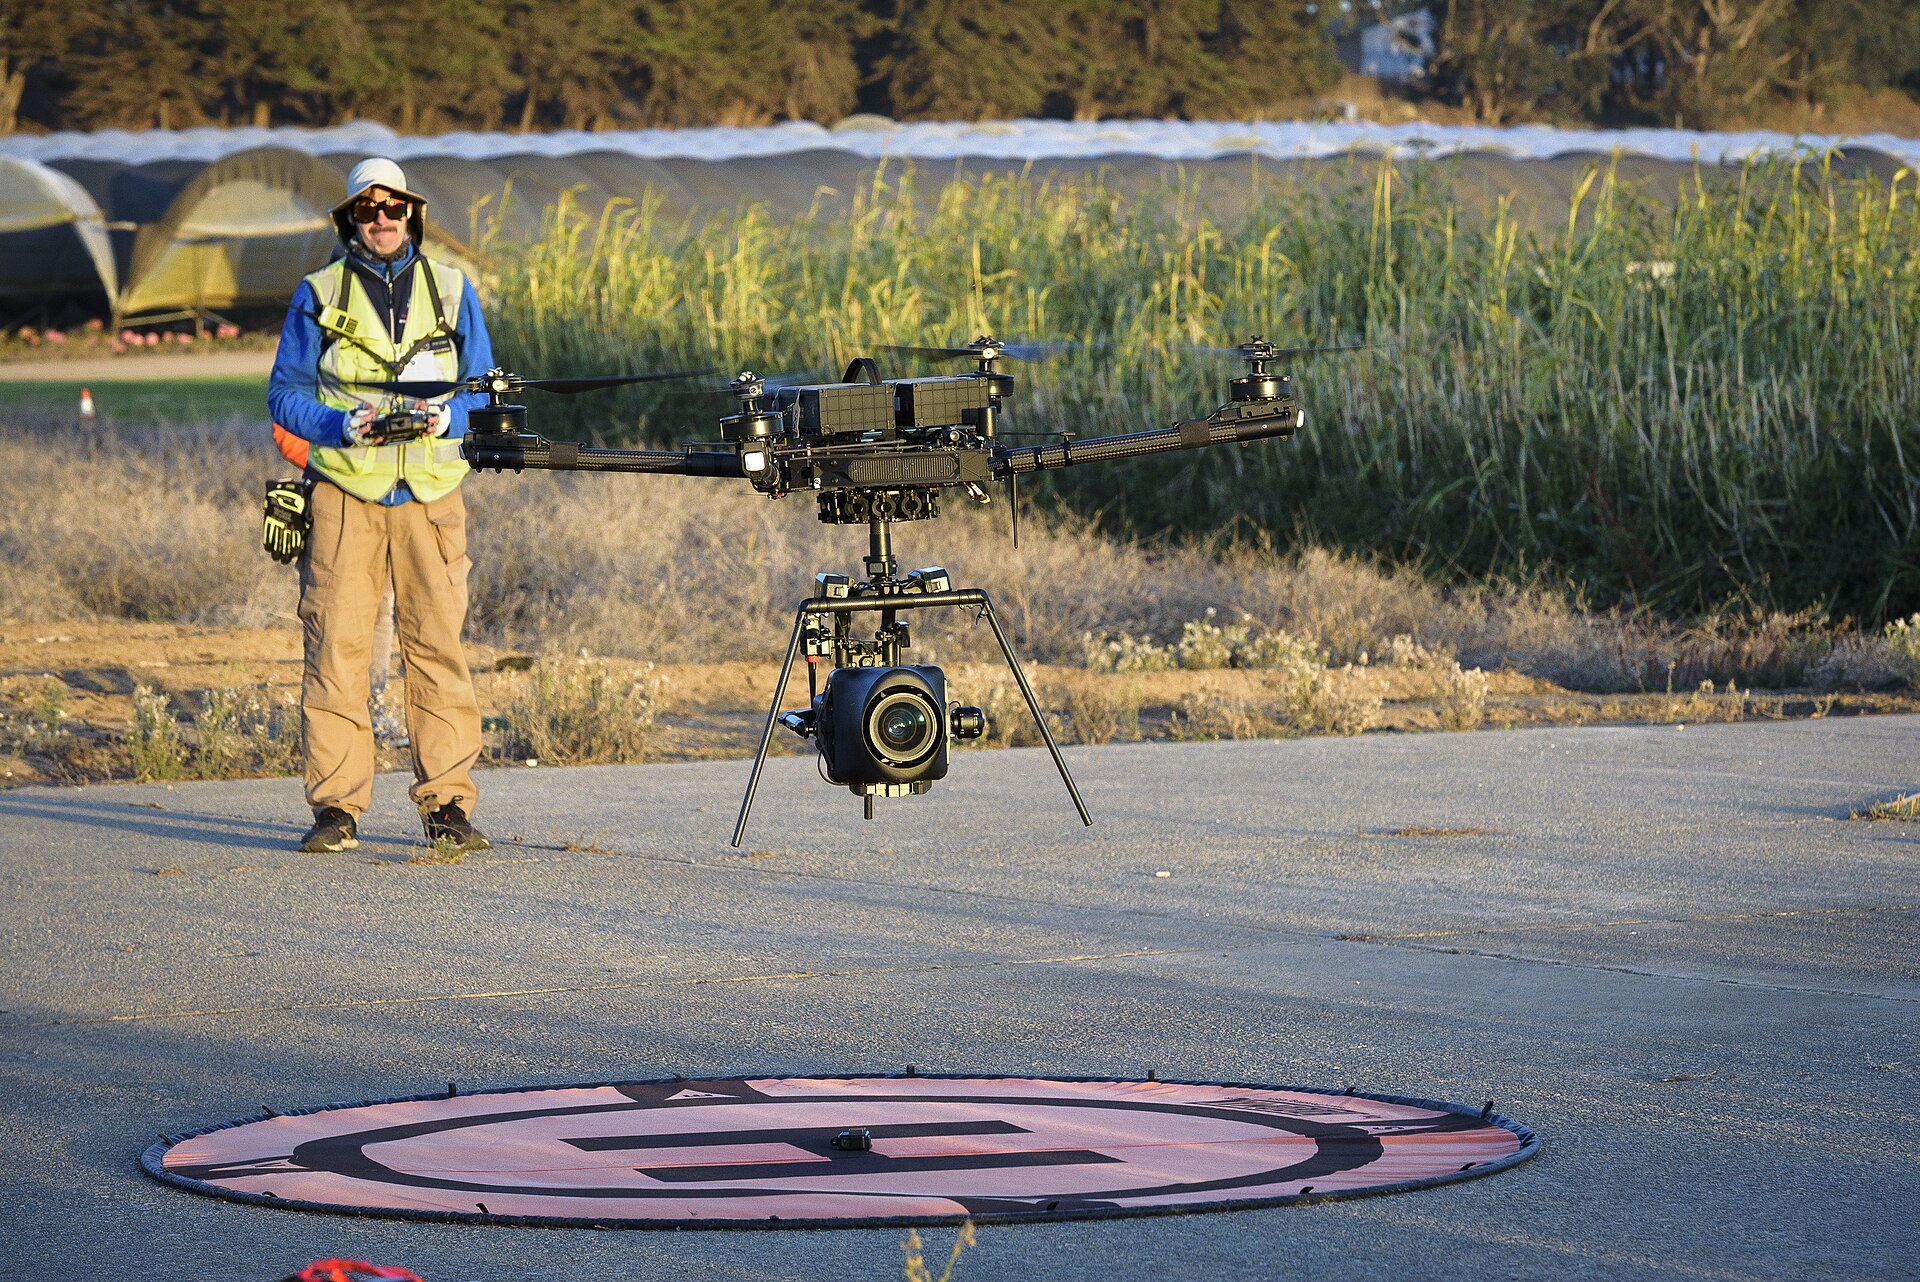
\includegraphics[width=\linewidth]{drone_landing_nasa.jpg}};
      \begin{scope}[x={(img.south east)},y={(img.north west)}]
        \tikzset{tag/.style={fill=ink,fill opacity=0.85,text opacity=1,text=white,
                             rounded corners=2pt,inner sep=2pt,font=\small}}
        % descent speed
        \draw[-{Latex[length=2.5mm]},line width=1.8pt,accent] (0.60,0.56) -- (0.60,0.33);
        \node[tag,right] at (0.61,0.45) {$\nu_z$};
        % depth from the drone's camera to the landing pad
        \draw[white,line width=1.2pt,dashed] (0.458,0.36) -- (0.458,0.13);
        \node[tag,left] at (0.445,0.245) {depth $Z$};
      \end{scope}
    \end{tikzpicture}\\[0.5mm]
    {\scriptsize A camera drone descending onto its landing pad\fnmark{*}}
    \column{0.44\textwidth}
    \begin{tcolorbox}[colback=ink,colupper=white,arc=3pt,boxrule=0pt]
      \centering\large
      $\displaystyle \tau=\frac{Z}{\nu_z}=\frac{1}{\rho\,\nu_z},\qquad \rho=\frac{1}{Z}$
    \end{tcolorbox}
    \begin{itemize}\small
      \item \alert{TTC}: seconds left before the camera reaches a point, if motion stays the same
      \item Only the \alert{ratio} $Z/\nu_z$ matters, so no metric scale is needed: a \alert{single camera} is enough
      \item Needed for landing, braking and dodging, where reacting \alert{fast} matters most
    \end{itemize}
  \end{columns}
  \footer{\fnitem{*}{Photo: NASA Ames Research Center / D.~Richey, public domain, via Wikimedia Commons.}}
\end{frame}

\begin{frame}{Event cameras: pixels that report changes, not frames}
  \begin{columns}[T,onlytextwidth]
    \column{0.64\textwidth}
    \centering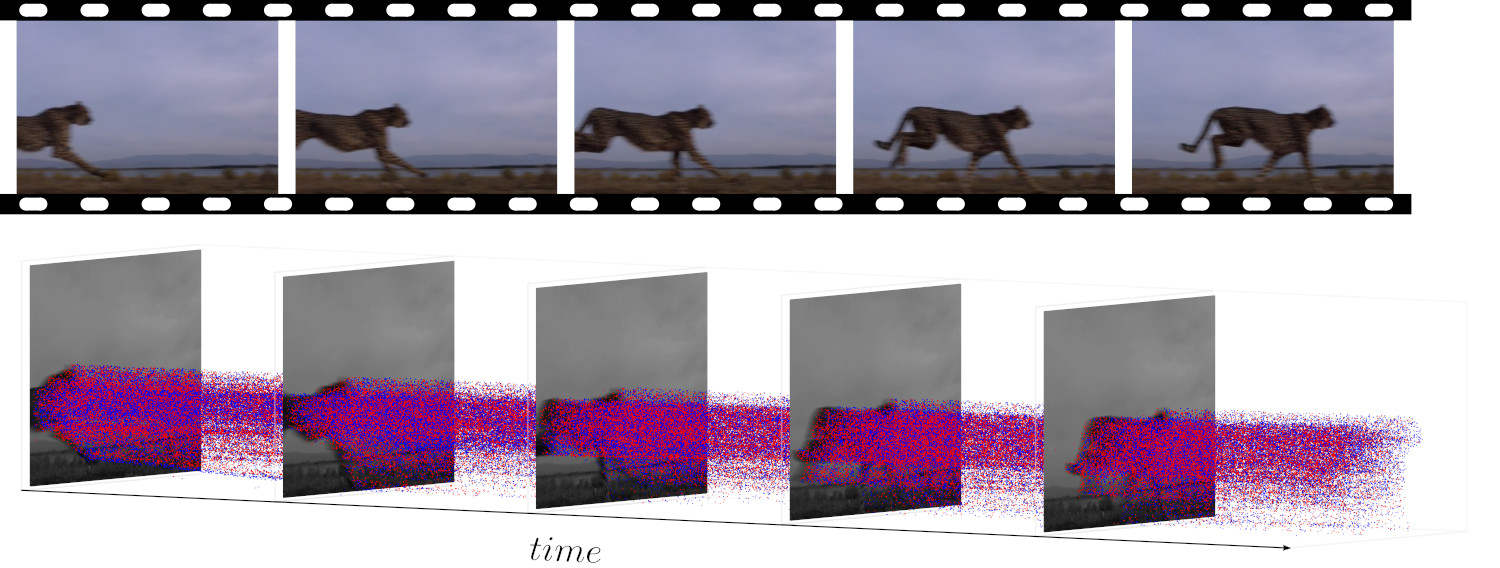
\includegraphics[width=0.9\linewidth]{event_camera_comparison.jpg}\\[0.5mm]
    {\scriptsize\textbf{Top:} frames at a fixed rate. \textbf{Bottom:} events of the same scene
     (\textcolor{red}{red}/\textcolor{blue}{blue} = brighter/darker).\fnmark{*}}

    \begin{itemize}\small\setlength{\itemsep}{1pt}
      \item Each pixel fires $e_i=(x_i,y_i,t_i,p_i)$ \alert{only when its brightness changes}: \alert{$\mu$s} resolution, no blur, high dynamic range, low power
      \item[\faExclamationTriangle] But there are \alert{no images}: methods must work on the event stream itself
    \end{itemize}
    \column{0.33\textwidth}
    \centering
    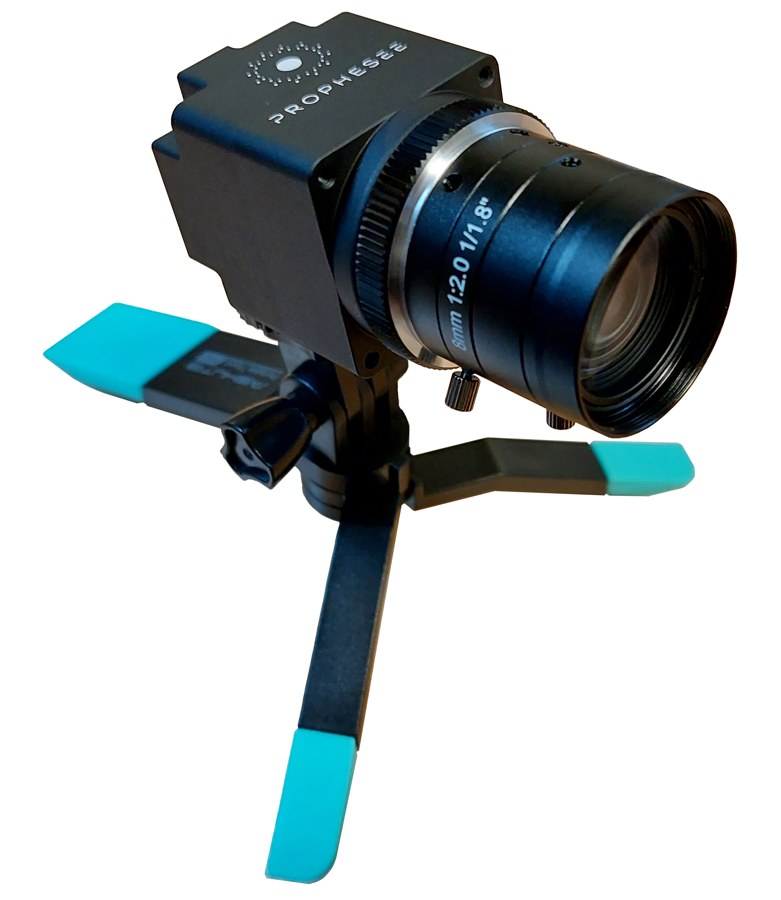
\includegraphics[height=0.52\textheight]{prophesee_evk.jpg}\\[1mm]
    {\footnotesize A real event camera (Prophesee),\\ the sensor type used for the VL dataset\fnmark{\dag}}
  \end{columns}
  \footer{\fnitem{*}{Image: T.~Stoffregen, CC BY-SA 4.0.}\quad
          \fnitem{\dag}{Photo: Auledas, CC BY 4.0. Both via Wikimedia Commons.}}
\end{frame}

% ================================================================= 2
\section{Why this paper is different}
\settag{2\enspace Why this paper is different}

\begin{frame}{The task, and how earlier methods did it}
  \begin{columns}[T,onlytextwidth]
    \column{0.49\textwidth}
    \begin{card}[equal height group=task]{accent}
      \textbf{Usual approach:} one \alert{global} TTC for the whole view, assuming the obstacle is
      \alert{planar and facing the camera}
    \end{card}
    \column{0.49\textwidth}
    \begin{card}[equal height group=task]{teal}
      \textbf{Goal here:} a \textbf{TTC map} (TTCM), one value per event/pixel, updated with
      \textbf{every event}, on a CPU (example: paper Fig.~5, slide~13)
    \end{card}
  \end{columns}

  \vspace{1mm}
  \centering\footnotesize\renewcommand{\arraystretch}{0.97}
  \begin{tabular}{@{}l l l l r r@{}}
    \toprule
    Method & Output & Assumption & HW & \us/event & REE (\%)\fnmark{\dag} \\
    \midrule
    PF \,[36]     & global TTC        & planar scene   & CPU & $\approx$1.9 & $\approx$40.6 \\
    E-RAFT \,[17] & flow (learned)    & training data  & GPU & $\approx$2.3 & $\approx$42.2 \\
    CT \,[43]     & global TTC        & planar scene   & CPU & $\approx$314 & $\approx$58.2 \\
    SOFAS \,[45]  & global TTC        & planar scene   & CPU & $\approx$486 & $\approx$34.8 \\
    ECMD \,[28]   & global divergence & planar scene   & GPU & 50.90 & 8.92 \\
    \midrule
    \rowcolor{good}\textbf{ETTCM} & \textbf{per-event TTC map} & one global motion & \textbf{CPU} & \textbf{1.15} & \textbf{5.64} \\
    \bottomrule
  \end{tabular}

  \vspace{0mm}
  \raggedright\small
  \begin{itemize}\setlength{\itemsep}{0pt}\setlength{\topsep}{2pt}
    \item ETTCM is \alert{36.8\,\%} more accurate than ECMD and \alert{95--98\,\%} faster ($\sim$40$\times$), with no GPU and no training;
      it also gives \alert{per-event optical flow} for free
  \end{itemize}
  \footer{\fnitem{\dag}{VL benchmark averages (paper Fig.~1, Table~2); $\approx$: read off the paper's Fig.~1.}}
\end{frame}

\begin{frame}{Runtime vs.\ accuracy (paper Fig.\ 1, re-made with our code)}
  \centering
  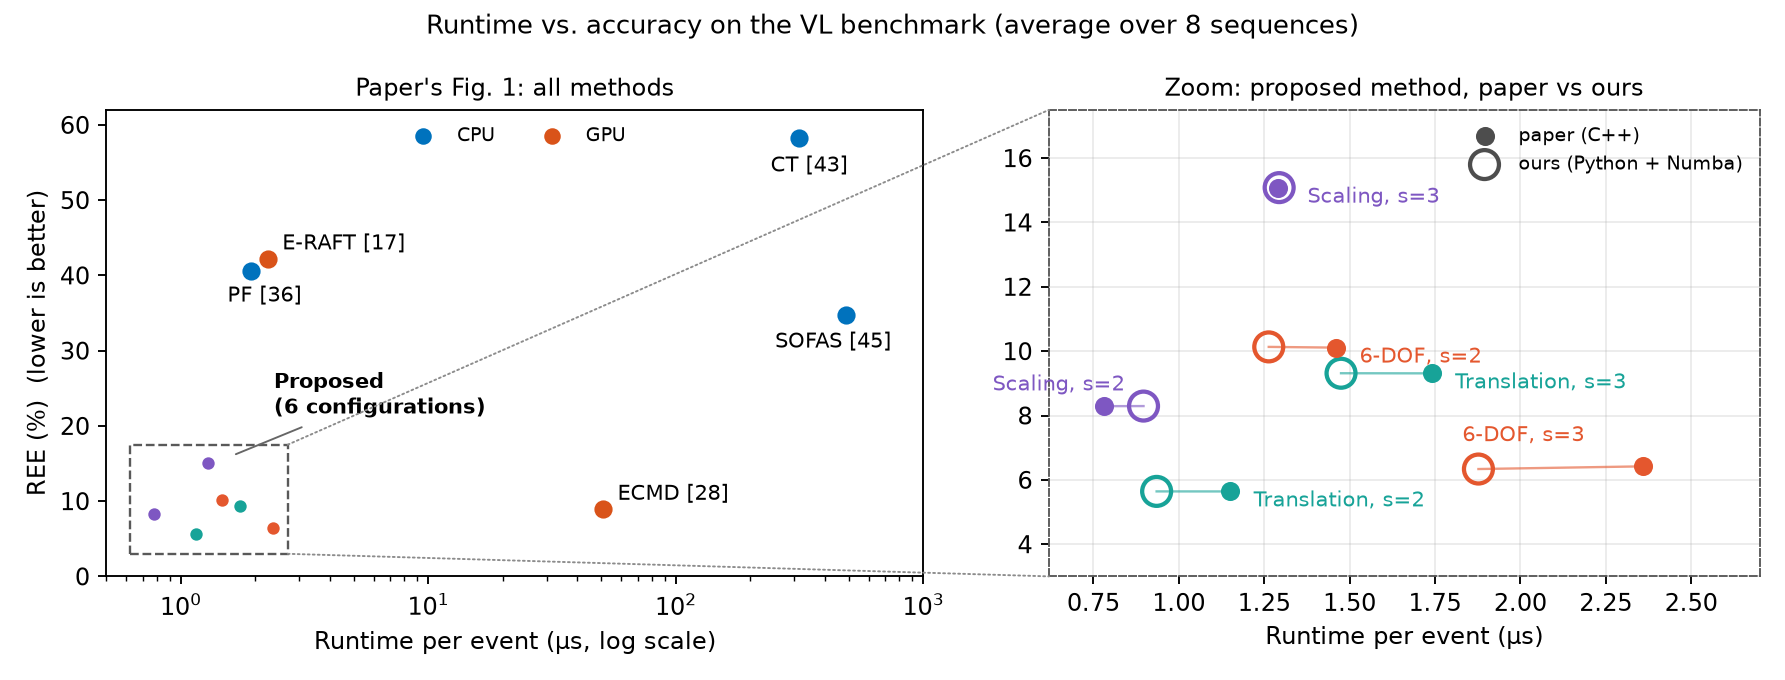
\includegraphics[width=\textwidth]{fig1_runtime.png}

  \vspace{1mm}
  \small Left: all TTC methods on the VL benchmark. Right: zoom on the proposed method;
  each of our six configurations (\textbf{hollow}) lands next to the paper's (\textbf{filled}):
  \alert{same error}, similar runtime (ours slightly faster on our laptop).
\end{frame}

% ================================================================= 3
\section{Use cases}
\settag{2\enspace Key ideas\quad 3\enspace Use cases}

\begin{frame}{Three key ideas, and where a fast TTC map is useful}
  \begin{columns}[T,onlytextwidth]
    \column{0.32\textwidth}
    \begin{card}[equal height group=ideas,fontupper=\footnotesize\raggedright]{accent}
      {\faProjectDiagram}\ \textbf{Joint local + global}\par\smallskip
      One \alert{global camera motion} $\bm\theta$ shared by all events, and a
      \alert{local inverse depth} $\rho_i$ for each event, estimated together
    \end{card}
    \column{0.32\textwidth}
    \begin{card}[equal height group=ideas,fontupper=\footnotesize\raggedright]{teal}
      {\faBolt}\ \textbf{Incremental}\par\smallskip
      One event at a time: small neighbourhood, $\le$\,2 Gauss--Newton steps,
      about \alert{1\us/event} on a CPU
    \end{card}
    \column{0.32\textwidth}
    \begin{card}[equal height group=ideas,fontupper=\footnotesize\raggedright]{ink}
      {\faIcon{compress-arrows-alt}}\ \textbf{No event collapse}\par\smallskip
      Neighbours are moved to the \alert{current event's time}, not a common reference,
      so scaling models cannot shrink everything to a point
    \end{card}
  \end{columns}

  \vspace{-1mm}
  {\color{titlebar}\bfseries Use cases}\par\vspace{-3mm}
  \begin{columns}[T,onlytextwidth]
    \column{0.49\textwidth}
    \begin{card}[equal height group=uses1,fontupper=\footnotesize\raggedright,after skip=1.5mm]{accent}
      \faHelicopter\ \textbf{Drone landing (ventral landing):}
      divergence of the ground below tells the drone when to slow down.
      \emph{VL benchmark, Tables 2 and 6.}
    \end{card}
    \begin{card}[equal height group=uses2,fontupper=\footnotesize\raggedright,before skip=0pt]{teal}
      \faPlane\ \textbf{Obstacle avoidance:}
      per-pixel TTC shows \emph{which} obstacle is closest in time, not just one global value.
      \emph{MVSEC indoor flying.}
    \end{card}
    \column{0.49\textwidth}
    \begin{card}[equal height group=uses1,fontupper=\footnotesize\raggedright,after skip=1.5mm]{ink}
      \faCar\ \textbf{Driving / collision warning:}
      dedicated \emph{Driving} motion model (forward speed + yaw) for cars.
      \emph{MVSEC outdoor\_day1.}
    \end{card}
    \begin{card}[equal height group=uses2,fontupper=\footnotesize\raggedright,before skip=0pt]{accent!70!ink}
      \faMicrochip\ \textbf{Embedded, low-power robots:}
      runs on a CPU at $\sim$1\us/event; sampling events (supp.\ Table~6) gives a further
      $\sim$9$\times$ speed-up with almost no loss.
    \end{card}
  \end{columns}
\end{frame}

% ================================================================= 4
\section{Methodology}
\settag{4\enspace Methodology}

\begin{frame}{From camera motion to flow, divergence and TTC}
  \begin{columns}[T,onlytextwidth]
    \column{0.56\textwidth}
    Image velocity of event $i$ (Eq.~9):
    \[
      \mathbf v_i=\rho_i\mathbf V_i\bm\nu+\bm\Omega_i\bm\omega=\mathbf B_i\bm\theta,
    \]
    \[
      \mathbf V_i=\begin{pmatrix}-f_x&0&x_i-c_x\\0&-f_y&y_i-c_y\end{pmatrix}
    \]
    Then for each event:
    \[
      \underbrace{\mu_i=\rho_i\,\nu_z}_{\text{divergence}}
      \qquad\Rightarrow\qquad
      \underbrace{\tau_i=1/\mu_i}_{\text{TTC}}
    \]
    \begin{itemize}\small
      \item $\rho$ and $\bm\nu$ are only known \alert{up to scale}: the method keeps $\|\bm\nu\|\le 1$
      \item The scale cancels in $\tau$, so TTC is still in \alert{seconds}
    \end{itemize}
    \column{0.40\textwidth}
    \small
    \begin{tabular}{@{}ll@{}}
      \toprule
      Motion model & Unknowns $\bm\theta$ \\
      \midrule
      Scaling & $\nu_z$ \\
      Translation & $\nu_x,\nu_y,\nu_z$ \\
      Driving & $\nu_z,\ \omega_y$ \;($|\nu_z|=1$) \\
      6-DOF & $\bm\nu,\ \bm\omega$ \\
      \bottomrule
    \end{tabular}

    \vspace{3mm}
    \footnotesize One global $\bm\theta$ shared by all events; one $\rho_i$ per event.
  \end{columns}
\end{frame}

\begin{frame}{The per-event pipeline}
  \centering
  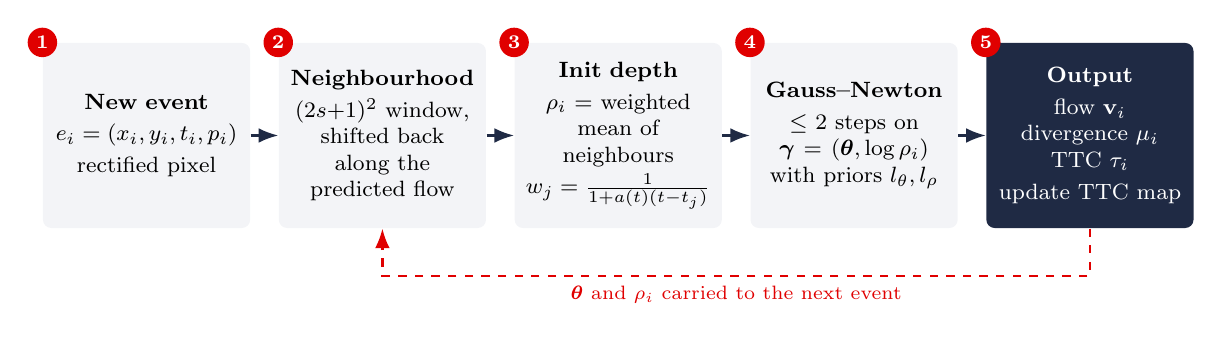
\begin{tikzpicture}[
      box/.style={draw=none,fill=soft,rounded corners=3pt,minimum height=2.35cm,
                  text width=2.35cm,align=center,font=\footnotesize,inner sep=4pt},
      num/.style={circle,fill=accent,text=white,font=\scriptsize\bfseries,inner sep=1.5pt},
      arr/.style={-{Latex[length=2.5mm]},thick,ink}]
    \node[box] (a) {\textbf{New event}\\[2pt] $e_i=(x_i,y_i,t_i,p_i)$\\[2pt] rectified pixel};
    \node[box,right=0.35cm of a] (b) {\textbf{Neighbourhood}\\[2pt] $(2s{+}1)^2$ window, shifted back along the predicted flow};
    \node[box,right=0.35cm of b] (c) {\textbf{Init depth}\\[2pt] $\rho_i$ = weighted mean of neighbours\\[2pt] $w_j=\frac{1}{1+a(t)(t-t_j)}$};
    \node[box,right=0.35cm of c] (d) {\textbf{Gauss--Newton}\\[2pt] $\le$ 2 steps on $\bm\gamma=(\bm\theta,\log\rho_i)$ with priors $l_\theta,l_\rho$};
    \node[box,right=0.35cm of d,fill=ink,text=white] (e) {\textbf{Output}\\[2pt] flow $\mathbf v_i$\\ divergence $\mu_i$\\ TTC $\tau_i$\\[2pt] update TTC map};
    \foreach \u/\v in {a/b,b/c,c/d,d/e} \draw[arr] (\u) -- (\v);
    \foreach \n/\k in {a/1,b/2,c/3,d/4,e/5} \node[num] at (\n.north west) {\k};
    \draw[arr,accent,dashed] (e.south) |- ++(0,-0.6) -| node[pos=0.25,below,font=\scriptsize] {$\bm\theta$ and $\rho_i$ carried to the next event} (b.south);
  \end{tikzpicture}

  \vspace{3mm}
  \small
  Cost: a few dozen neighbours $\times$ 2 iterations $\Rightarrow$ \alert{$\sim$1--2\us{} per event}, fast
  enough for MVSEC's peak of $\sim$400k events/s
\end{frame}

\begin{frame}{Dispersion minimisation without event collapse}
  \begin{columns}[c,onlytextwidth]
    \column{0.5\textwidth}
    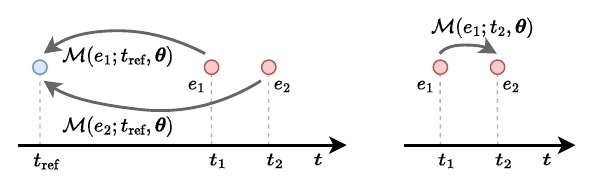
\includegraphics[width=\linewidth]{paper_fig3.png}\\
    {\scriptsize Common reference $t_\text{ref}$ (left) vs.\ local transform to $t_i$ (right)\fnmark{*}}

    \vspace{3mm}
    Update with priors (Eq.~8), $\mathbf L=\mathrm{diag}(l_\theta,\dots,l_\rho)$:
    \[ \Delta\bm\gamma=(\bm\Psi+\mathbf L)^{-1}\big(-\bm\psi+\mathbf L(\bm\gamma_\text{prev}-\bm\gamma)\big) \]
    \column{0.47\textwidth}
    Each neighbour $e_j$ is moved to the current time:
    \[ \mathbf r_{ij}=\mathbf x_i-\big(\mathbf x_j+\Delta t_{ij}\,\mathbf B_j\bm\theta\big) \]
    and $\sum_j w_{ij}\|\mathbf r_{ij}\|^2$ is minimised (Eq.~7).
    \begin{itemize}\small
      \item Small $\Delta t_{ij}$ $\Rightarrow$ constant-velocity assumption holds
      \item If $\bm\theta$ diverges, residuals grow, so \alert{collapse is penalised} without extra regularisers
    \end{itemize}
  \end{columns}
  \footer{\fnitem{*}{U.~M.~Nunes, L.~U.~Perrinet, S.-H.~Ieng, ICCV 2023, Fig.~3.}}
\end{frame}

% ================================================================= 5
\section{Experiments}
\settag{5\enspace Experiments}

\begin{frame}{Our re-implementation, datasets and metrics}
  \begin{columns}[T,onlytextwidth]
    \column{0.55\textwidth}
    \begin{itemize}\footnotesize\setlength{\itemsep}{0pt}
      \item \textbf{Python + Numba}, written from the paper and checked against the official C++
      \item \alert{Event-by-event identical} to the C++: median relative difference $\sim 10^{-7}$
      \item Official code only covers \textbf{Table 2}, so the \alert{MVSEC evaluation} (Tables 3--5, figures) is \textbf{our own}
      \item Streams 2--12 GB HDF5 files in chunks; 1--5\us/event
    \end{itemize}
    \column{0.42\textwidth}
    {\footnotesize\color{titlebar}\bfseries Settings (paper Table 1)}\par\vspace{0.5mm}
    \footnotesize\setlength{\tabcolsep}{4pt}\renewcommand{\arraystretch}{1.0}
    \begin{tabular}{@{}l c c c c c@{}}
      \toprule
      & $s$ & $w_\text{thresh}$ & $l_\theta$ & $l_\rho$ & GN iter. \\
      \midrule
      VL    & 2, 3 & 0.01 & 1000 & 1 & 2 \\
      MVSEC & 3    & 0.01 & 100  & 1 & 2 \\
      \bottomrule
    \end{tabular}\\[0.5mm]
    {\scriptsize $s$: neighbourhood; $l_\theta$, $l_\rho$: motion and depth priors}
  \end{columns}

  \vspace{0.5mm}
  \footnotesize\renewcommand{\arraystretch}{1.0}
  \begin{tabular}{@{}L{2.7cm}L{5.4cm}L{2.4cm}L{2.5cm}@{}}
    \toprule
    Dataset & Content & Ground truth & Used for \\
    \midrule
    \textbf{Ventral Landing} (VL) & 8 sequences (7 planar, 1 3D), Prophesee 1280$\times$720, 15\,s each & global divergence & Table~2, supp.\ Table~6, Figs.~1, 8 \\
    \textbf{MVSEC} & DAVIS 346$\times$260; indoor\_flying1--3 (drone) + outdoor\_day1 (car), 266\,s scored & depth, optical flow, camera velocity & Tables 3, 4, 5; Figs.~5, 6 \\
    \textbf{ECD} slider\_depth & DAVIS 240$\times$180, sliding camera & -- & Fig.~4 \\
    \bottomrule
  \end{tabular}

  \vspace{0.5mm}
  \begin{columns}[T,onlytextwidth]
    \column{0.49\textwidth}
    \begin{card}[equal height group=met,fontupper=\footnotesize\raggedright,top=2pt,bottom=2pt]{teal}
      \textbf{TTC / divergence:} REE (VL), AREE (MVSEC): mean of $|\hat\mu-\mu|/|\mu|$
    \end{card}
    \column{0.49\textwidth}
    \begin{card}[equal height group=met,fontupper=\footnotesize\raggedright,top=2pt,bottom=2pt]{accent}
      \textbf{Optical flow:} AEE (px), Out (\% $>$3\,px), AREE (\%), AAE (angle, $^\circ$)
    \end{card}
  \end{columns}
\end{frame}

\begin{frame}{Tables 2 and 6: TTC on Ventral Landing}
  \begin{columns}[T,onlytextwidth]
    \column{0.44\textwidth}
    {\color{titlebar}\bfseries Table 2}\par\vspace{1mm}
    \footnotesize\setlength{\tabcolsep}{4pt}
    \begin{tabular}{@{}l c r r r r@{}}
      \toprule
      & & \multicolumn{2}{c}{REE (\%) $\downarrow$} & \multicolumn{2}{c}{\us/event} \\
      \cmidrule(lr){3-4}\cmidrule(l){5-6}
      Model & $s$ & Paper & \textbf{Ours} & Paper & Ours \\
      \midrule
      Scaling     & 2 & 8.29  & \G\textbf{8.29}  & 0.78 & 0.90 \\
      Translation & 2 & 5.64  & \G\textbf{5.64}  & 1.15 & 0.94 \\
      6-DOF       & 2 & 10.11 & \G\textbf{10.13} & 1.46 & 1.26 \\
      Scaling     & 3 & 15.08 & \G\textbf{15.08} & 1.29 & 1.29 \\
      Translation & 3 & 9.31  & \G\textbf{9.31}  & 1.74 & 1.47 \\
      6-DOF       & 3 & 6.42  & \G\textbf{6.34}  & 2.36 & 1.88 \\
      \bottomrule
    \end{tabular}

    \vspace{2mm}
    \begin{card}[fontupper=\footnotesize\raggedright]{teal}
      \ok\ \textbf{Reproduced}: every average within 0.08 (each sequence within 0.6). Real-time on a laptop,
      like the paper. Baseline ECMD: 8.92\,\% at 50.9\us/event.
    \end{card}
    \column{0.54\textwidth}
    {\color{titlebar}\bfseries Supp.\ Table 6 / Fig.\ 8: fewer events, same accuracy}\par\vspace{1mm}
    \begin{minipage}[t]{0.6\linewidth}\vspace{0pt}
      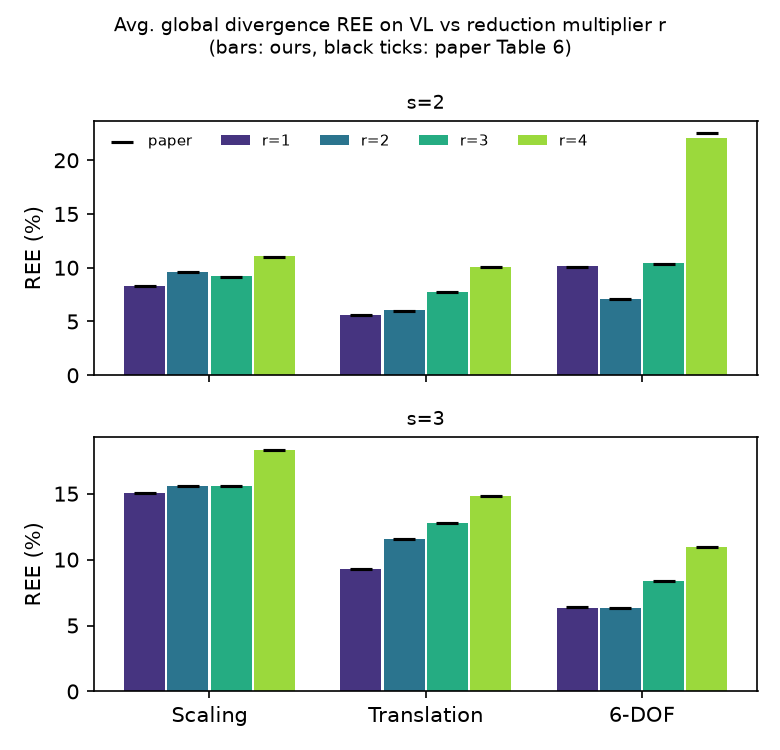
\includegraphics[width=\linewidth]{fig8_resolution.png}
    \end{minipage}\hfill
    \begin{minipage}[t]{0.37\linewidth}\vspace{0pt}
      \footnotesize\raggedright
      Divide coordinates by $r$; a counter per reduced pixel \alert{fires every $r^2$ events}\par\medskip
      $r=3$: \alert{11$\times$ fewer events}, accuracy almost unchanged\par\medskip
      Ported from the official \texttt{leaky\_\allowbreak sampling.hpp}
    \end{minipage}\par\vspace{1mm}
    \begin{card}[fontupper=\footnotesize\raggedright]{teal}
      \ok\ \textbf{Reproduced}: \textbf{23 of 24} averages within 0.08 of the paper
      (black ticks = paper)
    \end{card}
  \end{columns}
\end{frame}

\begin{frame}{Tables 4 and 5: optical flow on MVSEC}
  \centering\footnotesize\setlength{\tabcolsep}{3.5pt}\renewcommand{\arraystretch}{1.02}
  \adjustbox{max width=\textwidth}{%
  \begin{tabular}{@{}l l c c c c c c@{}}
    \toprule
    & & \multicolumn{4}{c}{\textbf{Table 4}: AEE (px) / Out (\%)} & \multicolumn{2}{c}{\textbf{Table 5}: AREE (\%) / AAE ($^\circ$)} \\
    \cmidrule(lr){3-6}\cmidrule(l){7-8}
    Model & & flying1 & flying2 & flying3 & outdoor & flying3 & outdoor \\
    \midrule
    \multirow{2}{*}{Driving} & Paper & 1.40 / 7.50 & 2.42 / 26.32 & 2.14 / 26.05 & 0.39 / 0.12 & 104.05 / 60.36 & 50.25 / 13.31 \\
    & \textbf{Ours} & \G 1.35 / 6.93 & \G 2.47 / 27.36 & \G 2.16 / 26.78 & \M 0.59 / 1.25 & \B 362.85 / \G 60.75 & \B 87.27 / \G 15.11 \\
    \midrule
    \multirow{2}{*}{Translation} & Paper & 0.63 / 0.41 & 0.94 / 2.83 & 0.79 / 1.65 & 0.55 / 0.97 & 44.46 / 11.38 & 72.67 / 21.77 \\
    & \textbf{Ours} & \G 0.66 / 0.87 & \M 1.19 / 6.48 & \M 0.94 / 3.69 & \M 0.67 / 1.59 & \M 50.90 / \G 12.12 & \M 92.73 / \G 21.95 \\
    \midrule
    \multirow{2}{*}{6-DOF} & Paper & 0.88 / 1.97 & 1.60 / 12.02 & 1.38 / 9.99 & 0.81 / 2.26 & 95.23 / 21.35 & 122.04 / 31.68 \\
    & \textbf{Ours} & \G 0.84 / 1.79 & \G 1.60 / 10.77 & \G 1.38 / 8.66 & \G 0.76 / 1.83 & \G 84.35 / \G 21.41 & \G 120.17 / \G 22.42 \\
    \bottomrule
  \end{tabular}}\\[0.8mm]
  {\scriptsize flying$k$ = indoor\_flying$k$,\quad outdoor = outdoor\_day1}

  \vspace{1mm}
  \begin{columns}[T,onlytextwidth]
    \column{0.28\textwidth}
    \begin{card}[equal height group=t45,fontupper=\footnotesize\raggedright]{teal}
      \ok\ \textbf{Table 4: 8 of 12} within 0.05\,px (Driving and 6-DOF indoors match almost exactly)
    \end{card}
    \column{0.28\textwidth}
    \begin{card}[equal height group=t45,fontupper=\footnotesize\raggedright]{accent!80!yellow}
      Translation 0.03--0.25\,px worse; a sweep of $s$, $l_\theta$ reaches 1.05, not 0.94
    \end{card}
    \column{0.40\textwidth}
    \begin{card}[equal height group=t45,fontupper=\footnotesize\raggedright]{accent}
      \textbf{Table 5: direction (AAE) reproduced everywhere.} AREE is off for Driving although its
      AEE matches, so the difference is in \alert{how near-zero ground truth was scored}
    \end{card}
  \end{columns}
\end{frame}

\begin{frame}{Table 3: divergence (TTC) on MVSEC, AREE \%}
  \centering\footnotesize\renewcommand{\arraystretch}{1.0}
  \begin{tabular}{@{}l l r r r@{}}
    \toprule
    Model & Scoring & indoor\_flying1 & indoor\_flying2 & outdoor\_day1 \\
    \midrule
    \multirow{3}{*}{Translation} & \textbf{Paper} & \textbf{19.82} & \textbf{28.23} & \textbf{45.78} \\
    & Ours, plain mean (Eq.~14) & \B 66.77 & \B 81.88 & \M 54.31 \\
    & Ours, median & \G 23.82 & \G 28.69 & \G 43.98 \\
    \midrule
    \multirow{3}{*}{6-DOF} & \textbf{Paper} & \textbf{53.65} & \textbf{56.12} & \textbf{56.66} \\
    & Ours, plain mean & \B 113.15 & \B 120.27 & \M 66.83 \\
    & Ours, median & \B 83.24 & \B 95.73 & \G 53.74 \\
    \midrule
    \multirow{3}{*}{Driving} & \textbf{Paper} & \textbf{153.30} & \textbf{84.80} & \textbf{47.27} \\
    & Ours, plain mean & \B 315.52 & \B 212.16 & \B 71.08 \\
    & Ours, median & \G 120.33 & \M 103.35 & \M 36.05 \\
    \bottomrule
  \end{tabular}

  \vspace{3mm}
  \begin{card}{accent}
    The drone often barely moves forward ($|V_z|<0.05$\,m/s in 13--20\,\% of frames): true divergence
    $\approx 0$, so a relative error explodes. With a median (or ignoring $|\mu|<0.2$/s) Translation
    \alert{matches}; the paper never says which rule it used.
  \end{card}
\end{frame}

\begin{frame}{Qualitative: Fig.\ 5 (TTC map) and Fig.\ 4 (depth)}
  \begin{columns}[T,onlytextwidth]
    \column{0.49\textwidth}
    \centering
    {\color{titlebar}\bfseries Fig.~5: TTC map, MVSEC indoor\_flying1}\\[1mm]
    {\footnotesize\textbf{Paper}\fnmark{*}}\\[0.5mm]
    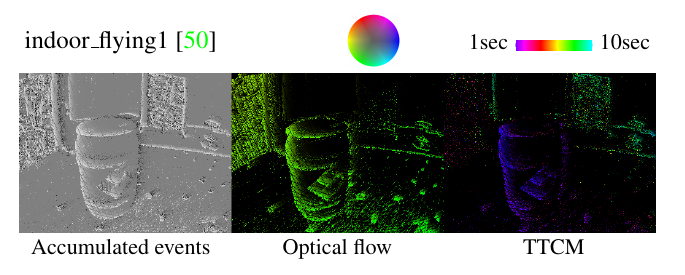
\includegraphics[width=0.72\linewidth]{paper_fig5.png}\\[0.5mm]
    {\footnotesize\textbf{Ours}}\\[0.5mm]
    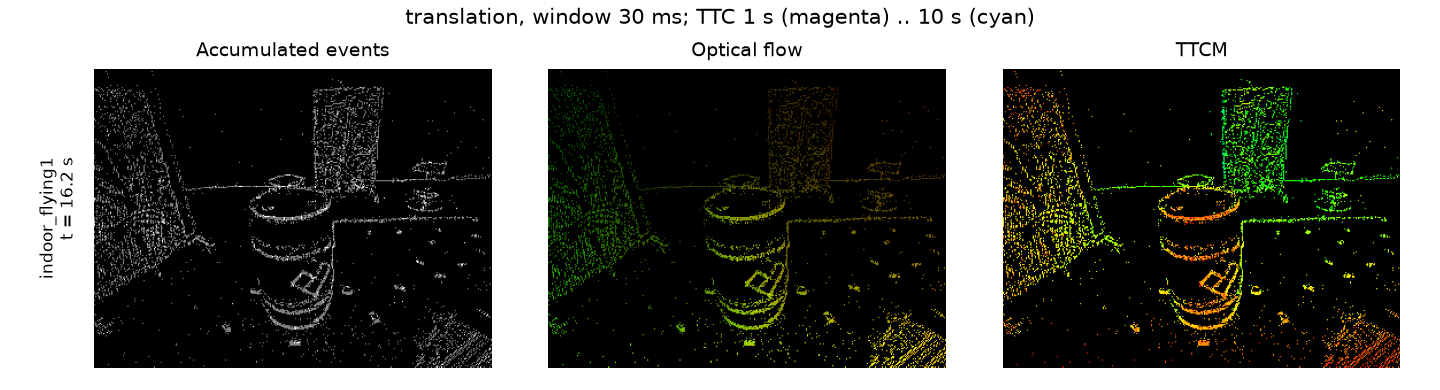
\includegraphics[width=0.94\linewidth]{fig5_if1.png}\\[0.5mm]
    \raggedright\footnotesize Same scene, same colour bar (1\,s magenta $\rightarrow$ 10\,s cyan):
    the barrel is closest in time (red/orange)
    \column{0.49\textwidth}
    \centering
    {\color{titlebar}\bfseries Fig.~4: depth, ECD slider\_depth}\\[1mm]
    {\footnotesize\textbf{Paper}\fnmark{*}}\\[0.5mm]
    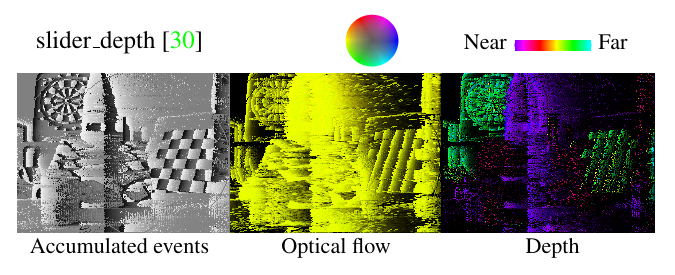
\includegraphics[width=0.72\linewidth]{paper_fig4.png}\\[0.5mm]
    {\footnotesize\textbf{Ours}}\\[0.5mm]
    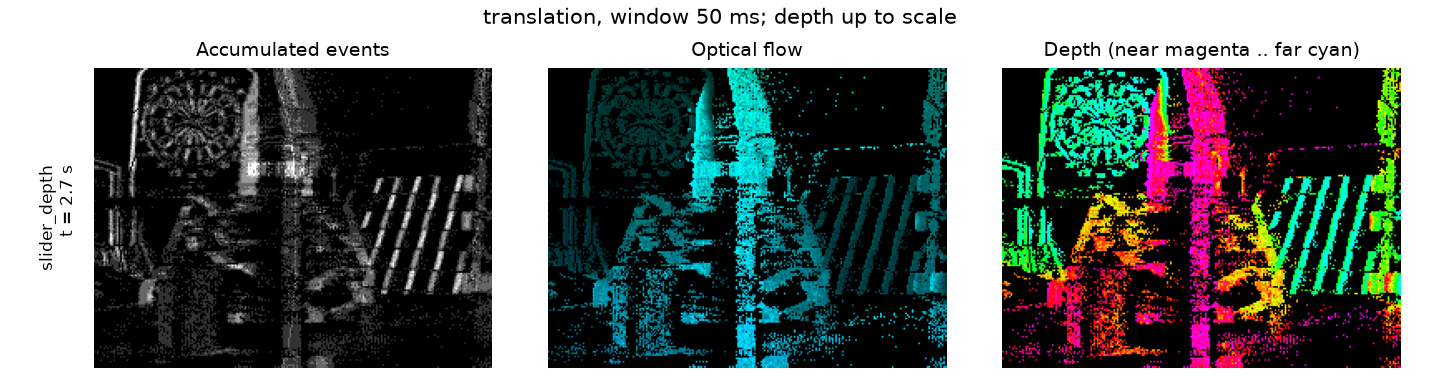
\includegraphics[width=0.94\linewidth]{fig4_slider_depth.png}\\[0.5mm]
    \raggedright\footnotesize Near objects magenta, far dartboard and checkerboard green/cyan, as in the paper
    (flow colours differ only by the colour-wheel convention)
  \end{columns}
  \footer{\fnitem{*}{U.~M.~Nunes, L.~U.~Perrinet, S.-H.~Ieng, ICCV 2023, Figs.~5 and 4.}}
\end{frame}

\begin{frame}{Qualitative: Fig.\ 6 (all MVSEC sequences)}
  \begin{columns}[T,onlytextwidth]
    \column{0.47\textwidth}
    \centering\textbf{Paper}\fnmark{*}\\[1mm]
    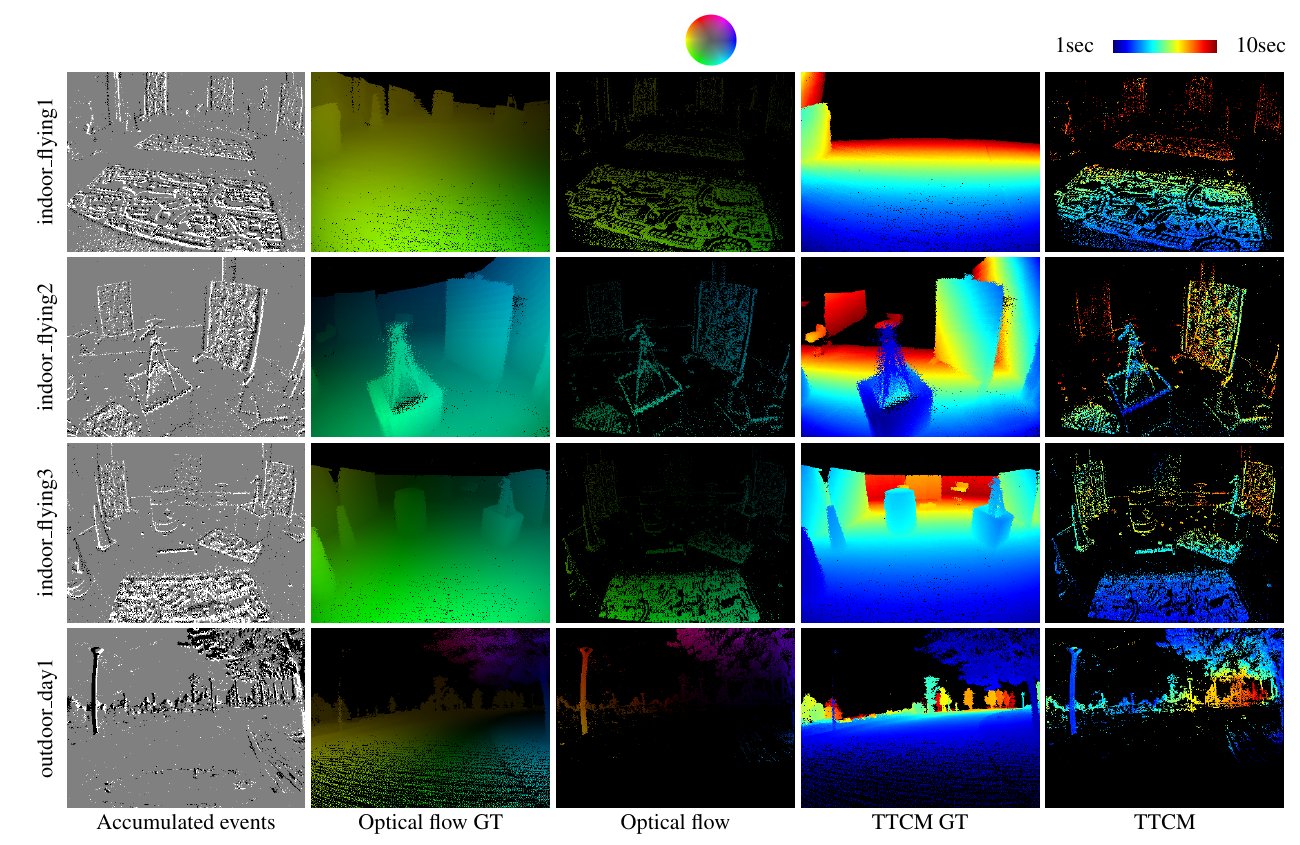
\includegraphics[width=0.92\linewidth]{paper_fig6.png}
    \column{0.51\textwidth}
    \centering\textbf{Ours} (Translation)\\[1mm]
    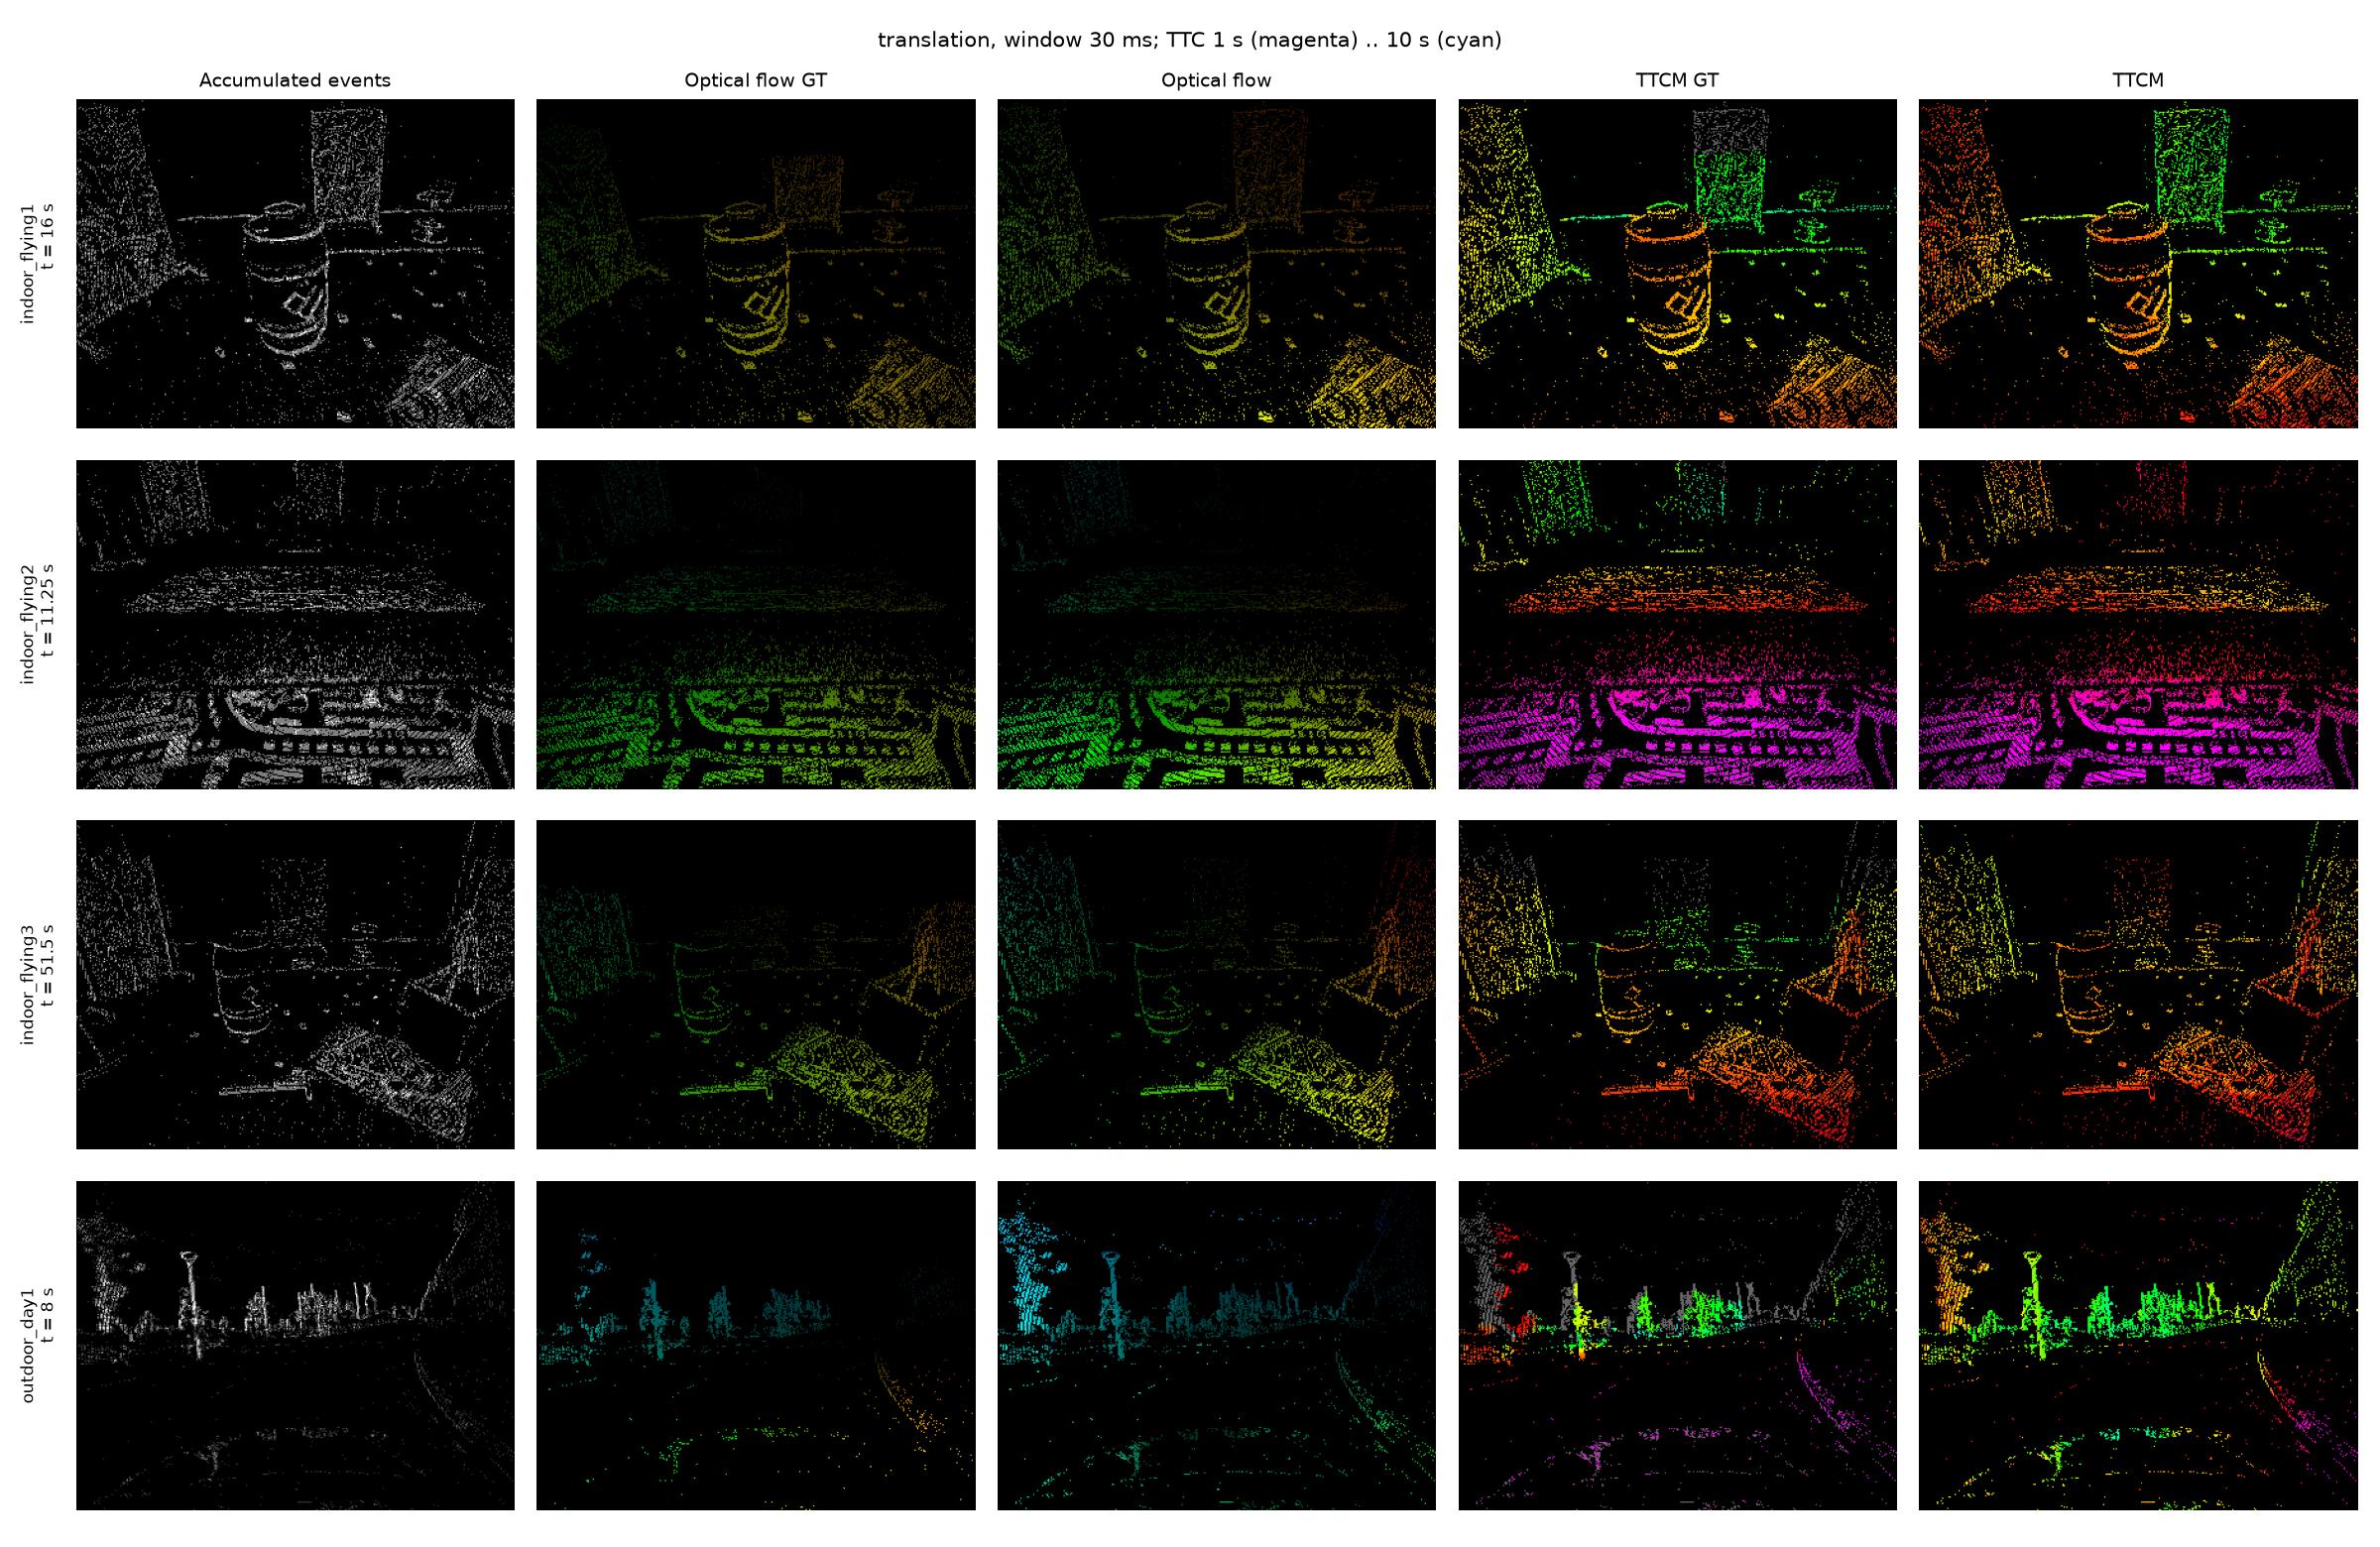
\includegraphics[width=0.92\linewidth]{fig6_translation.png}
  \end{columns}
  \vspace{2mm}
  \small
  Estimated flow and TTC maps \alert{follow the ground truth} on every sequence. Differences: the paper draws
  dense GT maps and a blue--red TTC scale; ours shows GT at event pixels with the Fig.~5 scale.
  Times not given in the paper, so we chose moments of strong forward motion.
  \footer{\fnitem{*}{U.~M.~Nunes, L.~U.~Perrinet, S.-H.~Ieng, ICCV 2023, Fig.~6.}}
\end{frame}

% ================================================================= 6
\section{What we did and how much we reproduced}
\settag{6\enspace What we did and how much}

\begin{frame}{What we built, and the problems we found (and fixed)}
  \begin{columns}[T,onlytextwidth]
    \column{0.39\textwidth}
    {\color{titlebar}\bfseries What we built}
    \begin{itemize}\footnotesize\setlength{\itemsep}{0pt}
      \item[\ok] Estimator, all \textbf{4 motion models}
      \item[\ok] Verified \textbf{event by event} against the official C++
      \item[\ok] VL: \textbf{Table 2}, \textbf{Fig.~1}; supplementary \textbf{Table 6}, \textbf{Fig.~8}
      \item[\ok] MVSEC pipeline from scratch: \textbf{Tables 3, 4, 5}; qualitative \textbf{Figs.~4, 5, 6}
      \item[\ok] Data checks, unit tests, scripts for every table
    \end{itemize}
    \begin{card}[fontupper=\footnotesize\raggedright,before skip=1mm]{ink}
      \textbf{Repository}\par
      \texttt{ettcm/} estimator, models, MVSEC I/O, sampling\\
      \texttt{scripts/} one script per table / figure\\
      \texttt{tests/} 5 test files, all pass\\
      \texttt{README.md}, \texttt{RESULTS.md}: every number, how to re-run, what we tried
    \end{card}
    \column{0.58\textwidth}
    {\color{titlebar}\bfseries Problems we found (and fixed)}\par\vspace{1mm}
    \footnotesize\renewcommand{\arraystretch}{1.05}
    \begin{tabular}{@{}>{\raggedright\arraybackslash}p{2.45cm}>{\raggedright\arraybackslash}p{5.45cm}@{}}
      \toprule
      Problem & Cause $\rightarrow$ fix \\
      \midrule
      6-DOF did not match the paper & Paper's 6-DOF is an \alert{undocumented re-parameterised model} in the C++ $\rightarrow$ ported it \\
      Small differences everywhere & Official build uses an \alert{approximate \texttt{exp()}} (up to 6\,\% off) $\rightarrow$ mirrored \\
      MVSEC flow did not line up & GT flow is in \alert{rectified} pixels despite the \texttt{\_dist} name $\rightarrow$ rectified camera \\
      463\,s scored instead of $\sim$265\,s & Wrong time windows $\rightarrow$ EV-FlowNet windows: 266\,s \\
      Divergence 2$\times$ too large & \leavevmode\alert{MVSEC's GT flow implies only 55--65\,\%} of the odometry speed $\rightarrow$ use odometry \\
      Outdoor Driving went backwards & Driving keeps the sign it starts with; car still at start $\rightarrow$ start forward \\
      \bottomrule
    \end{tabular}
  \end{columns}
\end{frame}

\begin{frame}{How much did we reproduce?}
  \begin{columns}[c,onlytextwidth]
    \column{0.56\textwidth}
    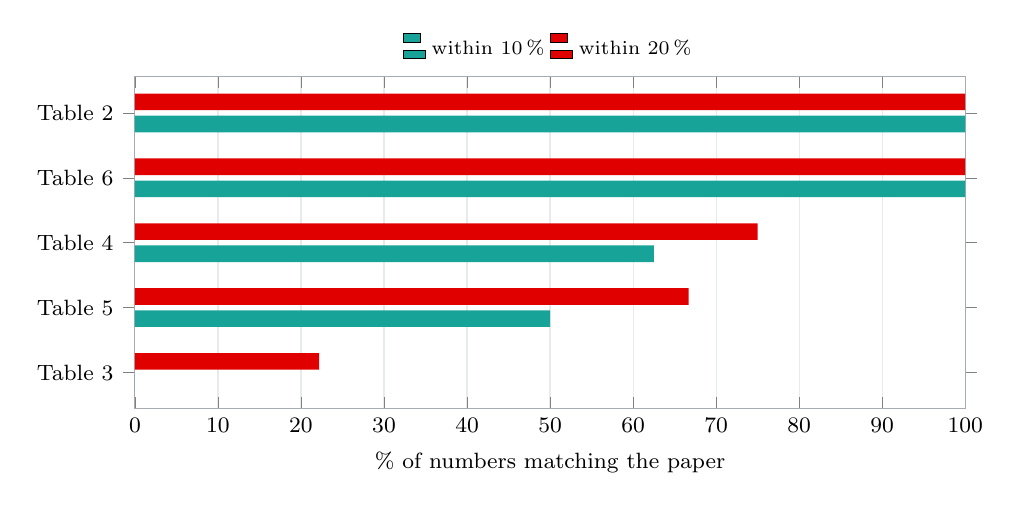
\begin{tikzpicture}
      \begin{axis}[
        xbar, width=\linewidth, height=5.8cm, xmin=0, xmax=100,
        bar width=6pt, enlarge y limits=0.14,
        symbolic y coords={Table 3,Table 5,Table 4,Table 6,Table 2},
        ytick=data,
        xlabel={\% of numbers matching the paper},
        tick label style={font=\footnotesize}, label style={font=\footnotesize},
        legend style={font=\scriptsize,at={(0.5,1.02)},anchor=south,draw=none,fill=none},legend columns=2,
        axis line style={ink!40}, xmajorgrids, grid style={ink!10}]
        \addplot[fill=teal,draw=none] coordinates {(0,Table 3) (50,Table 5) (62.5,Table 4) (100,Table 6) (100,Table 2)};
        \addplot[fill=accent,draw=none] coordinates {(22.2,Table 3) (66.7,Table 5) (75,Table 4) (100,Table 6) (100,Table 2)};
        \legend{within 10\,\%, within 20\,\%}
      \end{axis}
    \end{tikzpicture}
    \column{0.42\textwidth}
    \begin{tcolorbox}[colback=ink,colupper=white,boxrule=0pt,arc=3pt,halign=center]
      {\small by paper item}\\[2mm]{\Huge\bfseries $\approx$\,85\,\%}\\[2mm]
      {\small number by number: 65--77\,\%}\\
      {\small method itself: 100\,\% (matches the C++)}
    \end{tcolorbox}
    \footnotesize
    Items: Tables 2, 6, Figs.~1, 4, 5, 6, 8 full; Table 4 $\approx$\,0.75; Table 5 $\approx$\,0.5; Table 3 $\approx$\,0.3
    (8.5 of 10). Numbers: 69 values, Table 3 with the paper's literal formula.
  \end{columns}
\end{frame}

\begin{frame}{Why the remaining numbers differ, and conclusions}
  \begin{columns}[T,onlytextwidth]
    \column{0.51\textwidth}
    {\color{titlebar}\bfseries Why the remaining numbers differ}
    \begin{enumerate}\footnotesize\setlength{\itemsep}{1pt}
      \item \textbf{Scoring of near-zero ground truth} (Tables 3, 5)\\
        {\footnotesize Relative errors divide by the true value; the paper does not say how hovering frames were handled.
        Median / threshold rules make Translation match.}
      \item \textbf{Which 6-DOF Jacobian?} (Table 3, 6-DOF)\\
        {\footnotesize The released C++ \alert{differs from the paper's own Eq.~18} (supplementary). We tested both:
        Table~2 only matches the C++ one, and neither matches the MVSEC numbers.}
      \item \textbf{How outdoor\_day1 was run} (Driving: 0.59 vs 0.39\,px)\\
        {\footnotesize We ruled out the start point; settings are not given.}
    \end{enumerate}
    \begin{card}[fontupper=\footnotesize\raggedright,top=2pt,bottom=2pt,before skip=1mm]{teal}
      All three come from \textbf{evaluation details not in the paper}; we sent the questions to the authors.
      Everything the paper does specify is reproduced.
    \end{card}
    \column{0.46\textwidth}
    {\color{titlebar}\bfseries Conclusions}
    \begin{itemize}\footnotesize\setlength{\itemsep}{1pt}
      \item ETTCM gives a \alert{per-pixel TTC map} from a single event camera at $\sim$1\us/event on a CPU
      \item Our Python re-implementation is \alert{identical to the authors' code} event by event
      \item \textbf{VL results reproduced to rounding} (Tables 2, 6, Figs.~1, 8)
      \item \textbf{MVSEC optical flow mostly reproduced}; \textbf{divergence partly}, limited by unstated scoring
      \item By-product finding: \alert{MVSEC's GT flow and odometry disagree} on forward speed (55--65\,\%)
    \end{itemize}
    \begin{card}[fontupper=\footnotesize\raggedright,top=2pt,bottom=2pt,before skip=1mm]{accent}
      \textbf{Lesson:} a paper without its evaluation script cannot be fully reproduced, even when the method
      code is public.
    \end{card}
  \end{columns}
\end{frame}

\settag{}
\begin{frame}[standout]
  Thank you\\[3mm]
  {\large Questions?}
\end{frame}

% ================================================================= backup
\appendix
\settag{Backup}
\begin{frame}{Backup: Table 3 scoring rules, 6-DOF Jacobian, Translation sweep}
  \begin{columns}[T,onlytextwidth]
    \column{0.53\textwidth}
    \textbf{Table 3 scoring rules (indoor\_flying3)}\\[1mm]
    \footnotesize\setlength{\tabcolsep}{3.5pt}\renewcommand{\arraystretch}{1.02}
    \begin{tabular}{@{}>{\raggedright\arraybackslash}p{3.3cm} r r r@{}}
      \toprule
      Scoring rule & Driving & Transl. & 6-DOF \\
      \midrule
      all events, plain mean (Eq.~14) & 388.91 & 153.85 & 209.21 \\
      median & 105.59 & 24.52 & 87.49 \\
      errors capped at 100\,\% & 90.88 & 37.28 & 74.80 \\
      $|\mu_\text{gt}|\ge 0.1$/s (73\,\% kept) & 124.56 & 32.31 & 83.96 \\
      $|\mu_\text{gt}|\ge 0.2$/s (52\,\% kept) & 106.39 & 25.11 & 82.56 \\
      frames $|V_z|\ge 0.2$\,m/s & 125.63 & 30.51 & 86.24 \\
      TTC map at depth frames & 397.21 & 166.97 & 213.69 \\
      \bottomrule
    \end{tabular}

    \vspace{2mm}
    The paper's text says Driving does poorly on indoor\_flying3, but its Table 3 shows indoor\_flying2;
    indoor\_flying3 behaves like indoor\_flying2, so a label swap does not explain the gap.
    \column{0.44\textwidth}
    \textbf{6-DOF, official vs.\ consistent Jacobian}\\[1mm]
    \footnotesize\renewcommand{\arraystretch}{1.0}
    \begin{tabular}{@{}lrrr@{}}
      \toprule
      & Paper & Official & Consistent \\
      \midrule
      VL, $s=2$ & 10.11 & 10.13 & 5.72 \\
      VL, $s=3$ & 6.42 & 6.34 & 13.80 \\
      if1 AEE & 0.88 & 0.84 & 0.75 \\
      if2 AEE & 1.60 & 1.60 & 11.41 \\
      if3 AEE & 1.38 & 1.38 & 1.08 \\
      od1 AEE & 0.81 & 0.76 & 256.5 \\
      \bottomrule
    \end{tabular}

    \vspace{2mm}
    {\small\textbf{Translation, indoor\_flying2 AEE (paper 0.94)}}\\[1mm]
    \begin{tabular}{@{}lrrrrr@{}}
      \toprule
      $s$ \textbackslash\ $l_\theta$ & 30 & 100 & 300 & 1000 & 3000 \\
      \midrule
      2 & 11.6 & 9.71 & 7.01 & & \\
      3 & 1.27 & \textbf{1.19} & 1.07 & 1.05 & 1.05 \\
      4 & 1.17 & 1.11 & 1.07 & 1.06 & 1.06 \\
      \bottomrule
    \end{tabular}\\[1mm]
    Bold: the paper's settings. Levels off at 1.05.
  \end{columns}
\end{frame}

\end{document}
